\clearpage\section{Chapter 4: Advanced Language Features}
The previous chapters described a wide range of built-in computational
facilities that comprise much of what makes Unicon a great language.
This chapter delves into interesting features that help make Unicon
more than just the sum of its parts. This chapter demonstrates the
following tasks:

\begin{itemize}
\item Controlling expressions more precisely
\item Using list structures and procedure parameter lists
interchangeably
\item Holding a \index{generator}generator expression in a value so that
its results can be used in different locations throughout the program
\item Defining your own \index{control structure}control structures
\item Evaluating several generator expressions in parallel
\item Permuting strings using sophisticated mappings
\end{itemize}
\subsection[Limiting or Negating an Expression]{Limiting or Negating an
Expression}
\index{limiting an expression}Chapter 1 described generators and the
expression mechanism without mentioning many methods for using them,
other than \textsf{every} loops. Suppose you wish to generate five
elements from a table. If the table has thousands of elements, then you
may want to generate just five elements precisely in a situation where
generating all the table elements with \textsf{!T} is infeasible. You
could write an \textsf{every} loop that breaks out after five
iterations, but this solution isn{\textquotesingle}t easy to use within
some more complex expressions. The binary backslash operator
\textsf{\textit{expr}}\textsf{ {\textbackslash} }\textsf{\textit{i}}
limits \textsf{\textit{expr}} to at most \textsf{\textit{i}} results.
If \textsf{expr} has fewer results, the limitation operator has no
effect; once \textsf{\textit{i}} results have been obtained, limitation
causes the expression to \index{expression failure}fail even if it
could produce more results.

Unicon does not have a boolean type, so it might not have surprised you
that Chapter 1 downplayed the standard logical operators. The
\index{alternation operator ( {\textbar} )}alternation operator
(\textsf{{\textbar}}) resembles a short-circuit \index{OR operator}OR
operator, since it generates its left operand and only evaluates its
right operand if the left operand or the surrounding expression fails.
The conjunction operator (\textsf{\&}) resembles a short-circuit
\index{AND operator}AND operator, since it evaluates its left operand,
and if that operand succeeds, then the result of the conjunction is the
result of its right operand. The reserved word \textsf{not} rounds out
the boolean-like operators. If \textsf{\textit{expr}} produces no
results, then \index{not}\textsf{not }\textsf{\textit{expr}} will
succeed (and produce a null value); if \textsf{\textit{expr}} produces
any results, then the \textsf{not} expression fails. The \textsf{not}
operator can remedy certain forms of generator confusion. Compare the
following two expressions:

\iconcode{
if not (s ==
({\textquotedbl}good{\textquotedbl}{\textbar}{\textquotedbl}will{\textquotedbl}{\textbar}{\textquotedbl}hunting{\textquotedbl}))
then write({\textquotedbl}nope{\textquotedbl})}

\iconcode{
if (s \~{}==
({\textquotedbl}good{\textquotedbl}{\textbar}{\textquotedbl}will{\textquotedbl}{\textbar}{\textquotedbl}hunting{\textquotedbl}))
then write({\textquotedbl}uh huh{\textquotedbl})}

The first expression uses \textsf{not} to ensure that string \textsf{s}
is none of the three words. The second expression always writes
\textsf{{\textquotedbl}uh huh{\textquotedbl}}, because any string
\textsf{s} that you pick will be not equal (\textsf{\~{}==}) to at
least one of the three strings in the alternation. The \textsf{then}
part will always execute, which is probably not what was intended.

{\sffamily\bfseries
Note}

{\sffamily
Negating an == operator is not the same as using a \~{}== operator. You
have been warned!}

The \index{conjunction \&}conjunction operator
\textsf{\textit{expr}}\textsf{\textit{\textsubscript{1}}}\textsf{ \&
}\textsf{\textit{expr}}\textsf{\textit{\textsubscript{2}}} has an
alternate syntax, a comma-separated list of expressions in parentheses:
\textsf{(}\textsf{\textit{expr}}\textsf{\textit{\textsubscript{1}}}\textsf{
, }\textsf{\textit{expr}}\textsf{\textit{\textsubscript{2}}}\textsf{)}.
Any number of expressions may be present, and the whole expression only
succeeds if they all succeed. This looks similar to the syntax for a
procedure call because it is similar: a procedure call mutually
evaluates all the actual parameters before the procedure is invoked.
Besides putting a procedure value in front of a parenthesized argument
list, you can put a string or an integer. For a string value, as in
\textsf{s(x)}, a procedure by the name given in \textsf{s} is called;
if \textsf{s} had the value \textsf{{\textquotedbl}foo{\textquotedbl}},
then \textsf{s(x)} is the same as \textsf{foo(x)}. For an integer value
\textsf{i}, after all arguments are evaluated, the value of the entire
expression is the value of the \textsf{i}{\textquotesingle}th argument.

\subsection{List Structures and Parameter Lists}
The functions \textsf{write()} and \textsf{put()} take any number of
arguments; this flexibility helps make them powerful and convenient.
You can write \index{variable!no. of arguments}variable argument
procedures of your own by ending the last parameter in your procedure
declaration with empty square brackets:

\iconcode{
procedure myfunc(x, y, z[])}

In this case, instead of throwing away all arguments after the third,
the third parameter and all parameters that follow are placed into a
newly-constructed list. If you called the above procedure with
\textsf{myfunc(1, 2, 3, 4, 5)}, then \textsf{z} would have the value
\textsf{[3, 4, 5]}.

It is also useful to go the other direction and construct a list data
structure of dynamic (or user-supplied) length, and then call a
procedure with that list as its parameter list. The
\index{list!invocation}\index{apply operator}apply operator, binary
\textsf{!} performs this feat. If you call \textsf{write ! L}, then all
the elements of \textsf{L} are written contiguously on a single line
(unless they contain newline characters).

\subsection{Co-expressions}
A \index{co-expression}co-expression is an independent, encapsulated
\index{thread}thread{}-like context, where the results of an expression
(hopefully a generator!) can be picked off one at a time. Let us
consider an example. Suppose you are writing a program that generates
code, and you need something that will generate unique variable names.
This expression will generate names:

\iconcode{
{\textquotedbl}name{\textquotedbl} {\textbar}{\textbar} seq()}

The \index{seq()}\textsf{seq()} function produces an infinite sequence
of integers, by default starting at 1, so the whole expression
generates the sequence \textsf{{\textquotedbl}name1{\textquotedbl}},
\textsf{{\textquotedbl}name2{\textquotedbl}},
\textsf{{\textquotedbl}name3{\textquotedbl}}, ... and so forth. You can
put this expression at some point in your code; but you may need to use
it from several different places.

There are times when you need to separate the evaluation of an
expression from its textual position in the program. The normal
mechanism to do this would be a procedure. You can make separate calls
to a procedure from different locations in your program, but there is
no easy way to use the results from a single \index{instance}instance
of a generator in multiple locations. You can put all the results in a
list (not a good idea for generators with infinite result sequences) or
rewrite the procedure to produce the sequence using separate calls, but
this requires static or global variables, and is awkward at best. Here
is a crude effort

\iconcode{
procedure nameseq() \\
static i \\
initial i := 0 \\
\>   return {\textquotedbl}name{\textquotedbl} {\textbar}{\textbar} (i
+:= 1) \\
end
}

Now, consider the code generating program example again. It may need not
a single name sequence, but two kinds of names: statement labels and
temporary variables. In this case, you will have to write a different
procedure for each such sequence you need. The \textsf{nameseq()}
procedure was already cumbersome for so simple a task, but generalizing
it for multiple kinds of names makes it \textit{really} messy. By
creating a pair of co-expressions, you can capture exactly what is
needed with a lot less code:

\iconcode{
labelname := create ({\textquotedbl}\_L{\textquotedbl}
{\textbar}{\textbar} seq()) \\
varname := create({\textquotedbl}\_V{\textquotedbl} {\textbar}{\textbar}
seq())
}

In both cases, \index{create}\textsf{create}\textsf{
}\textsf{\textit{expr}} allocates and initializes an evaluation context
plus the memory needed to evaluate expression \textit{expr}, but does
not start to evaluate it. Since the co-expression value may be used
outside the procedure call where it is created, the evaluation context
has to include a copy of the local variables and parameters used in the
expression. When a co-expression is \textit{activated}, it produces the
next value. A co-expression is activated by the @ operator. Each
activation of \textsf{labelname} will produce the next string in the
sequence \textsf{{\textquotedbl}\_L0{\textquotedbl}},
\textsf{{\textquotedbl}\_L1{\textquotedbl}},
\textsf{{\textquotedbl}\_L2{\textquotedbl}}, and so on. Similarly, each
activation \textsf{@varname}\textsf{ }produces the next in the sequence
\textsf{{\textquotedbl}\_V0{\textquotedbl}},
\textsf{{\textquotedbl}\_V1{\textquotedbl}},
\textsf{{\textquotedbl}\_V2{\textquotedbl}}, and so on. 

\iconcode{
loop\_name := @labelname \\
tempvar\_name := @varname
}

After a co-expression has produced all its results, further evaluation
with \textsf{@} will \index{fail!co-expression}fail. The \textsf{\^{}}
operator produces a new co-expression with the same expression as its
argument, but {\textquotedbl}rewound{\textquotedbl} to the beginning.

\iconcode{
\>   c := \^{}c}

\subsection[User{}-Defined Control Structures]{User-Defined Control
Structures}
\index{control structure}Control structures are those elements of a
language that determine in what order, and how many times, expressions
are executed. Co-expressions can be used to implement new
\textit{control structures} in the sense that procedures that take
co-expression arguments as parameters can control the order and number
of times their arguments are activated.

Consider a control structure that selects values from the first
expression at the positions specified by the second. This could be
invoked as:

\iconcode{
seqsel([create fibonacci(), create primes()])}

Assuming that you have a pair of \index{generator}generator procedures
that produce the Fibonacci numbers (1, 1, 2, 3, 5, 8, 13, \ ?) and the
primes (2, 3, 5, 7, 11, ?), this expression produces the numbers 1, 2,
5, 13, 89, ....

Here is the implementation of \textsf{seqsel()}:

\iconcode{
procedure seqsel(a) \\
\>   (*a = 2) {\textbar} stop({\textquotedbl}seqsel requires a list of
two arguments{\textquotedbl}) \ \ \ \# We need two arguments \\
\>   e1 := a[1]; e2 := a[2] \\
\ \ \ \# position in the first stream we are looking at \\
\>   index := 1 \\
\>   repeat \{ \\
\>   \ \ \ \# Get the next index \\
\>   \ \ \ (i := @e2 ) {\textbar} fail \\
\ \ \ \ \ \ \# Keep getting values from the second expression until \\
\ \ \ \ \ \ \# we get to the i{\textquotesingle}th one. If e1 cannot produce that \\
\ \ \ \ \ \ \# many values, we fail. \\
\>   \ \ \ every index to i do \\
\>   \ \ \ (value := @e1) {\textbar} fail \\
\>   \ \ \ suspend value \\
\>   \ \ \ index := i+1 \\
\>   \ \ \ \} \\
end
}

Unicon provides a syntactic short-cut for this kind of usage:

\iconcode{
proc([create e1, create e2, ..., create en])
}

\noindent
can also be written with curly brackets, as

\iconcode{
proc\{e1, e2, ..., en\}
}

\subsection[Parallel Evaluation]{Parallel Evaluation}

\index{parallel evaluation}Co-expressions can be used to evaluate
expressions {\textquotedbl}in parallel{\textquotedbl} or in lock-step.
This program writes a table of \index{ASCII}ASCII characters with the
hex, decimal, and octal equivalents:

\iconcode{
procedure main() \\
\>   dec := create(0 to 255) \\
\>   hex\_dig := {\textquotedbl}0123456789abcdef{\textquotedbl} \\
\>   hex := create(!hex\_dig {\textbar}{\textbar} !hex\_dig) \\
\>   oct := create((0 to 3) {\textbar}{\textbar} (0 to 7)
{\textbar}{\textbar} (0 to 7)) \\
\>   char := create image(!\&cset) \\
\>   while write(@dec, {\textquotedbl}{\textbackslash}t{\textquotedbl},
@oct, {\textquotedbl}{\textbackslash}t{\textquotedbl}, @hex,
{\textquotedbl}{\textbackslash}t{\textquotedbl}, @char) \\
end
}

Co-expression \textsf{dec} produces the sequence 0, 1, 2, ... 255;
\textsf{hex} the sequence \textsf{{\textquotedbl}00{\textquotedbl}},
\textsf{{\textquotedbl}01{\textquotedbl}},
\textsf{{\textquotedbl}03{\textquotedbl}}, ...
\textsf{{\textquotedbl}ff{\textquotedbl}}; \textsf{oct}\textsf{ }the
sequence \textsf{{\textquotedbl}001{\textquotedbl}},
\textsf{{\textquotedbl}002{\textquotedbl}}, ...
\textsf{{\textquotedbl}377{\textquotedbl}}; and \textsf{char}\textsf{
}the sequence ..., \textsf{{\textquotedbl} {\textquotedbl}},
\textsf{{\textquotedbl}!{\textquotedbl}}, ...,
\textsf{{\textquotedbl}A{\textquotedbl}}, ...
\textsf{{\textquotedbl}Z{\textquotedbl}}, ...,
\textsf{{\textquotedbl}a{\textquotedbl}}, ...
\textsf{{\textquotedbl}z{\textquotedbl}}, and so forth.

Every invocation of \textsf{write()} results in all the co-expressions
being activated once, so they are all run in lock-step, producing this
table:

{\sffamily
0 \ \ \ \ \ \ 000 \ \ \ \ 00
\ \ \ \ \ {\textquotedbl}{\textbackslash}x00{\textquotedbl}}

{\sffamily
1 \ \ \ \ \ \ 001 \ \ \ \ 01
\ \ \ \ \ {\textquotedbl}{\textbackslash}x01{\textquotedbl}}

{\sffamily
2 \ \ \ \ \ \ 002 \ \ \ \ 02
\ \ \ \ \ {\textquotedbl}{\textbackslash}x02{\textquotedbl}}

{\sffamily
...}

{\sffamily
45 \ \ \ \ \ 055 \ \ \ \ 2d \ \ \ \ \ {\textquotedbl}-{\textquotedbl}}

{\sffamily
46 \ \ \ \ \ 056 \ \ \ \ 2e \ \ \ \ \ {\textquotedbl}.{\textquotedbl}}

{\sffamily
47 \ \ \ \ \ 057 \ \ \ \ 2f \ \ \ \ \ {\textquotedbl}/{\textquotedbl}}

{\sffamily
48 \ \ \ \ \ 060 \ \ \ \ 30 \ \ \ \ \ {\textquotedbl}0{\textquotedbl}}

{\sffamily
49 \ \ \ \ \ 061 \ \ \ \ 31 \ \ \ \ \ {\textquotedbl}1{\textquotedbl}}

{\sffamily
50 \ \ \ \ \ 062 \ \ \ \ 32 \ \ \ \ \ {\textquotedbl}2{\textquotedbl}}

{\sffamily
...}

{\sffamily
90 \ \ \ \ \ 132 \ \ \ \ 5a \ \ \ \ \ {\textquotedbl}Z{\textquotedbl}}

{\sffamily
91 \ \ \ \ \ 133 \ \ \ \ 5b \ \ \ \ \ {\textquotedbl}[{\textquotedbl}}

{\sffamily
92 \ \ \ \ \ 134 \ \ \ \ 5c
\ \ \ \ \ {\textquotedbl}{\textbackslash}{\textbackslash}{\textquotedbl}}

{\sffamily
93 \ \ \ \ \ 135 \ \ \ \ 5d \ \ \ \ \ {\textquotedbl}]{\textquotedbl}}

{\sffamily
94 \ \ \ \ \ 136 \ \ \ \ 5e
\ \ \ \ \ {\textquotedbl}\^{}{\textquotedbl}}

{\sffamily
95 \ \ \ \ \ 137 \ \ \ \ 5f \ \ \ \ \ {\textquotedbl}\_{\textquotedbl}}

{\sffamily
96 \ \ \ \ \ 140 \ \ \ \ 60
\ \ \ \ \ {\textquotedbl}{\textasciigrave}{\textquotedbl}}

{\sffamily
97 \ \ \ \ \ 141 \ \ \ \ 61 \ \ \ \ \ {\textquotedbl}a{\textquotedbl}}

{\sffamily
98 \ \ \ \ \ 142 \ \ \ \ 62 \ \ \ \ \ {\textquotedbl}b{\textquotedbl}}

{\sffamily
...}

{\sffamily
255 \ \ \ \ 377 \ \ \ \ ff
\ \ \ \ \ {\textquotedbl}{\textbackslash}xff{\textquotedbl}}

\noindent
Parallel evaluation can also be used to assign to a set of variables:

\iconcode{
ce := create !stat(f)}

\iconcode{
every (dev {\textbar} ino {\textbar} mode {\textbar} lnk {\textbar} uid
{\textbar} gid) := @ ce}

{\sffamily\bfseries
Note}

{\sffamily
stat() returns file information. It is presented in the next chapter.}

Coexpression creation can be quite expensive. This is probably not a
good way to assign a series of values to a group of variables but it
demonstrates an interesting technique.

\subsection{Coroutines}
In a conventional procedure invocation, procedures have an asymmetric
relationship; when control is transferred from the caller to the
callee, the callee procedure starts execution at the top. Coroutines
have an equal relationship: when control is transferred from one
coroutine to another, execution starts from the previous point that its
execution was suspended from. This process is called resumption. The
\index{producer/consumer}producer/consumer problem is a good example of
procedures that have an equal relationship. Figure 4-1 shows how the
control flow between coroutines is different from that of conventional
procedures.

{\centering \par}

\begin{center}
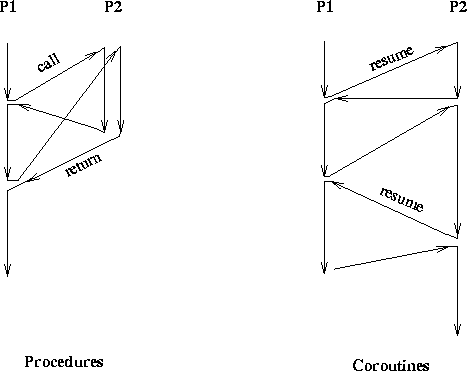
\includegraphics[width=3.9902in,height=3.1701in]{ub-img/ub-img8.png}
\end{center}

{\sffamily\bfseries Figure 4-1:}
{\sffamily The Difference Between Procedures and Coroutines}

\bigskip

Can you tell what the next example computes from its integer
command-line argument?

\bigskip

{\sffamily\bfseries
Listing 4-1}

{\sffamily\bfseries
Producer and Consumer Coroutines}

\iconcode{
procedure main(args) \\
\>   C1 := create consumer(args[1]) \\
\>   C2 := create producer(C1) \\
\>   @C2 \\
end \\
\ \\
procedure producer(ce) \\
\>   x := 1 \\
\>   repeat \{ \\
\>   \ \ \ val := x \^{} 2 \\
\>   \ \ \ ret := val @ ce {\textbar} break \\
\>   \ \ \ x +:= 1 \\
\>   \ \ \ \} \\
\>   @ \&main \\
end \\
\ \\
procedure consumer(limit) \\
\>   value := @ \&source \\
\>   repeat \{ \\
\>   \ \ \ \# process value \\
\>   \ \ \ if value {\textgreater} limit then break \\
\>   \ \ \ if value \% 2 = 0 then write(value) \\
\>   \ \ \ value := retval @ \&source \\
\>   \ \ \ \} \\
end
}

When producer resumes consumer, it passes \textsf{value}; the consumer
passes a return code (\textsf{retval}) back. \textsf{\&source} is the
coexpression that activated the current co-expression.

{\sffamily\bfseries
Note}

{\sffamily
This example doesn{\textquotesingle}t mean the producer/consumer problem
should always be done with coroutines!}

\subsubsection[Permutations]{Permutations}

\index{permutations}We have seen one usage of
\index{map()}\textsf{map()}, where it transformed mixed-case strings to
all lowercase. In that type of usage, the first string \ is the one
that we are manipulating, and the other two arguments tell it how the
string is to be modified. Interesting results can be achieved by
treating the \textit{third} argument as the string to manipulate.
Consider this code:

\iconcode{
s := {\textquotedbl}abcde{\textquotedbl} \\
write(map({\textquotedbl}01234{\textquotedbl},
{\textquotedbl}43201{\textquotedbl}, s))
}

What does this code example do? The transformation is:
\textsf{{\textquotedbl}4{\textquotedbl}} should be mapped to
\textsf{{\textquotedbl}a{\textquotedbl}},
\textsf{{\textquotedbl}3{\textquotedbl}} to
\textsf{{\textquotedbl}b{\textquotedbl}},
\textsf{{\textquotedbl}2{\textquotedbl}} to
\textsf{{\textquotedbl}c{\textquotedbl}},
\textsf{{\textquotedbl}0{\textquotedbl}} to
\textsf{{\textquotedbl}d{\textquotedbl}}, and
\textsf{{\textquotedbl}1{\textquotedbl}} to
\textsf{{\textquotedbl}e{\textquotedbl}}. When this mapping is applied
to \textsf{{\textquotedbl}01234{\textquotedbl}}, we get
\textsf{{\textquotedbl}edcab{\textquotedbl}} - a permutation of the
string \textsf{s}! It is exactly the permutation that is suggested by
the first two arguments of \textsf{map()}. To arrange this sort of
permutation, all three strings must be the same size, and there must be
no repeated letters in the second string.


\begin{center}
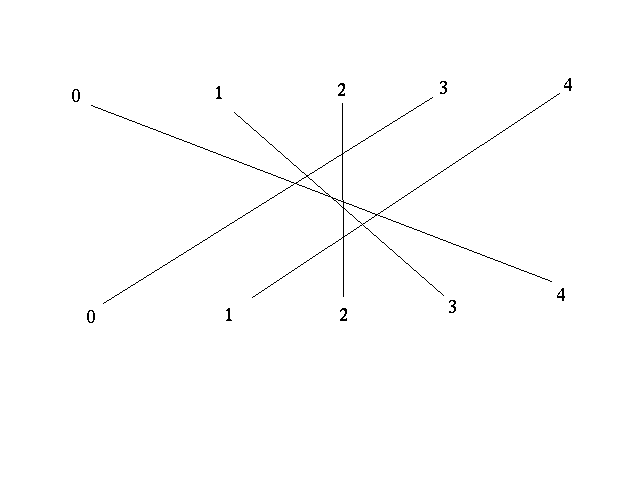
\includegraphics[width=5.0in,height=1.8in]{ub-img/ub-img9.png}
\end{center}
{\sffamily\bfseries Figure 4-2:}
{\sffamily Permuting a string with the map() function}

\bigskip

Here is an example: In the USA, dates are represented with the month
coming first, as in 12/25/1998, but in many other places the day comes
first: 25/12/1998. This conversion is, of course, just a permutation;
we can do this with a simple map:

\iconcode{
map({\textquotedbl}Mm/Dd/XxYy{\textquotedbl},
{\textquotedbl}Dd/Mm/XxYy{\textquotedbl}, date)
}

Here is another example. Unicon has a built-in random facility, the
\textsf{?} operator. Applied to a string or cset, it returns a random
character from the argument; applied to a structure, a random member of
that structure; and applied to an integer, a random integer between 1
and that number. This is a very useful feature and allows us to write
programs that shuffle cards or run simulations of things like rolling
dice.

By default in Unicon, the random sequence generated by \textsf{?} is
different for each run of the program. This is one of the few areas
where Unicon is deliberately different from Icon, which uses the same
seed each run by default. Icon{\textquotesingle}s semantics is good
when debugging, because we want the program to behave predictably while
it is broken! However, in most applications that use random numbers,
such as games, different runs of the program should create different
numbers. The \index{random!number seed}random number seed is keyword
\textsf{\&random.} It can be assigned a value at the start of main() in
order to get Icon-style repeatability. Here{\textquotesingle}s how to
assign it a number based on the current date and time.
Unicon{\textquotesingle}s default semantics do something similar.

\iconcode{
\&random := map({\textquotedbl}sSmMhH{\textquotedbl},
{\textquotedbl}Hh:Mm:Ss{\textquotedbl}, \&clock) +
map({\textquotedbl}YyXxMmDd{\textquotedbl},
{\textquotedbl}YyXx/Mm/Dd{\textquotedbl}, \&date)
}

The calls to \textsf{map()} remove punctuation characters from the
fixed-format strings produced by \textsf{\&clock} and \textsf{\&date}.
The resulting strings of digits are converted to integers, added, and
stored as a seed in \textsf{\&random}. Now every time the program is
run, the random number facility will be initialized with a different
number.

\subsection{Simulation}
A Galton Box is a device that demonstrates how balls falling through a
lattice of pegs will end up distributed binomially. A simulation of a
Galton box combines several of the techniques described previously.
\ Figure 4-3 is an illustration of the program{\textquotesingle}s
screen.



\begin{center}
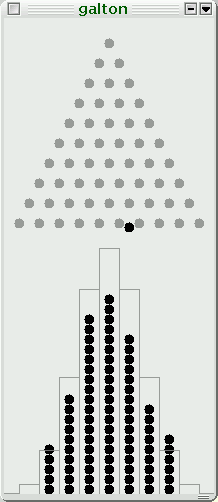
\includegraphics[width=1.75in,height=3.8201in]{ub-img/ub-img10.png}
\end{center}

{\sffamily\bfseries Figure 4-3:}
{\sffamily A Galton Box Simulation}

\bigskip

The simulation{\textquotesingle}s output window is a good example of
Unicon{\textquotesingle}s high-level graphics facilities. Graphics is a
broad area, discussed in Chapter 7 of this book; the on-line references
or the Icon graphics book (Griswold, Jeffery, Townsend 1998) contain
substantial additional details. Graphics are part of the system
interface. Some of the graphics functions used in this example include:

\begin{itemize}
\item \textsf{FillArc(x,y,width,height)} fills an ellipse defined by a
bounding rectangle. The shape is filled by the current foreground color
and/or fill pattern. The height defaults to be the same as the width,
producing a circle. Given additional arguments, \textsf{FillArc()
}fills parts of an ellipse similar to pieces of a pie in shape.
\item \textsf{WAttrib({\textquotedbl}attr{\textquotedbl})} or
\textsf{WAttrib({\textquotedbl}attr=value{\textquotedbl})}, the generic
routine for getting or setting a window{\textquotesingle}s attributes.
In this case the attributes \textsf{fg} (foreground color) and
\textsf{drawop} (raster drawing operation) are set to various colors
and reversible output.
\item \textsf{Window({\textquotedbl}attr=value{\textquotedbl}, ...)}
opens a window with initial characteristics as specified by a string of
attribute values. The \textsf{WDelay(t)} function waits until
\textsf{t} milliseconds have passed. The \textsf{WDone()} function
waits for the user to dismiss the output window by pressing
\textsf{{\textquotedbl}q{\textquotedbl}} and then terminates the
program and closes the window.
\end{itemize}
Listing 4-2 contains the code for a simplified version of the
simulation. A couple elements of the image above are omitted in order
to make the example easy to follow. (Both this program and the one that
created the screen shot above are included on the
book{\textquotesingle}s web site, http://unicon.sourceforge.net/book/)

{\sffamily\bfseries Listing 4-2}
{\sffamily\bfseries A Simple Galton Box Simulation}

\iconcode{
link graphics \\
global pegsize, height, width, pegsize2 \\
\ \\
procedure main(args) \\
local n, steps \\
\>   steps := 10 \\
\>   pegsize := 10 \\
\>   pegsize2 := pegsize * 2 \\
\>   n := integer(args[1]) {\textbar} 100 \\
\>   setup\_window(steps) \\
\>   every 1 to n do galton(steps) \\
\>   WDone() \\
end \\
\ \\
procedure setup\_window(n) \\
\ \\
local max, xpos, ypos, i, j \\
\>   \# Draw the n levels of pegs \\
\>   \# Pegboard size is 2n-1 square \\
\>   \# Expected max value of histogram is (n, n/2)/2\^{}n  \\
\>   \# ... approximate with something simpler? \\
\>   max := n*n/pegsize \\
\>   width := (2*n+1)*pegsize \\
\>   height := width + n*n/2*pegsize \\
\>   Window({\textquotedbl}size={\textquotedbl} {\textbar}{\textbar}
width {\textbar}{\textbar} {\textquotedbl},{\textquotedbl}
{\textbar}{\textbar} height, \\
\>   \ \ \ \ \ \ \ {\textquotedbl}fg=grayish-white{\textquotedbl}) \\
\>   WAttrib({\textquotedbl}fg=dark-grey{\textquotedbl}) \\
\>   every i := 1 to n do \{ \\
\>   \ \ \ ypos := i * pegsize2 \\
\>   \ \ \ xpos := width/2 - (i - 1) * pegsize - pegsize/2 \\
\>   \ \ \ every j := 1 to i do \{ \\
\>   \ \ \ \ \ \ FillArc(xpos, ypos, pegsize, pegsize) \\
\>   \ \ \ \ \ \ xpos +:= pegsize2 \\
\>   \ \ \ \ \ \ \} \\
\>   \ \ \ \} \\
\>   \# Set up drawing mode to draw the falling balls \\
\>   WAttrib({\textquotedbl}fg=black{\textquotedbl}) \\
\>   WAttrib({\textquotedbl}drawop=reverse{\textquotedbl}) \\
end
\ \\
\# Do it! \\
procedure galton(n) \\
local xpos, ypos, oldx, oldy \\
\>   xpos := oldx := width/2 - pegsize/2 \\
\>   ypos := oldy := pegsize \\
\>   \# For every ball... \\
\>   every 1 to n do \{ \\
\>   \ \ \ if ?2 = 1 then \\
\>   \ \ \ \ \ \ xpos -:= pegsize \\
\>   \ \ \ else \\
\>   \ \ \ \ \ \ xpos +:= pegsize \\
\>   \ \ \ ypos +:= pegsize2 \\
\>   \ \ \ animate(oldx, oldy, xpos, ypos) \\
\>   \ \ \ oldx := xpos \\
\>   \ \ \ oldy := ypos \\
\>   \ \ \ \} \\
\>   \# Now the ball falls to the floor \\
\>   animate(xpos, ypos, xpos, ypos + 40) \\
\ \ \ animate(xpos, ypos+40, xpos, ypos + 200) \\
\>   \# Record this ball \\
\>   draw\_ball(xpos) \\
end
\ \\
procedure animate(xfrom, yfrom, xto, yto) \\
\>   animate\_actual(xfrom, yfrom, xto, yfrom, 4) \\
\>   animate\_actual(xto, yfrom, xto, yto, 10) \\
end
\ \\
\# Drawing op is already set to {\textquotedbl}reverse{\textquotedbl},
and fg colour is black. \\
procedure animate\_actual(xfrom, yfrom, xto, yto, steps) \\
local x, y, xstep, ystep, i, lastx, lasty \\
\>   x := xfrom \\
\>   y := yfrom \\
\>   xstep := (xto - xfrom)/steps \\
\>   ystep := (yto - yfrom)/steps \\
\>   every i := 1 to steps do \{ \\
\>   \ \ \ lastx := x \\
\>   \ \ \ lasty := y \\
\>   \ \ \ FillArc(x, y, pegsize, pegsize) \\
\>   \ \ \ WDelay(1) \\
\>   \ \ \ FillArc(x, y, pegsize, pegsize) \\
\>   \ \ \ x +:= xstep \\
\>   \ \ \ y +:= ystep \\
\>   \ \ \ \} \\
end
\ \\
procedure draw\_ball(x) \\
static ballcounts \\
initial ballcounts := table(0) \\
\>   ballcounts[x] +:= 1 \\
\>   FillArc(x, height-ballcounts[x]*pegsize, pegsize, pegsize) \\
end
}

{\sffamily
Summary}

Unicon is particularly powerful when different language features are
combined. The ability to combine features in interesting ways is the
result of its novel expression semantics. Co-expressions add
substantial value to the concept of \index{generator}generators,
although most programs use them only sparingly. They fit well into a
philosophy that says that simple things should be easy to do...and
complex things should be easy to do as well.

